\def\r{3em}
\def\angle{10}
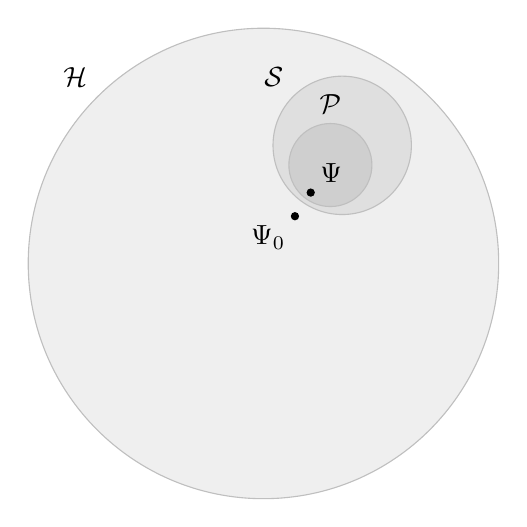
\begin{tikzpicture} 
	
	\node[
	name=H,
	circle,
	draw=lightgray,
	text=black,
	fill=lightgray!25,
	minimum size=17em
	] 
	(H) at (0,0) {};
	
	\node[anchor=south east] at (H.north west)
	{$\mathcal{H}$};
	
	\node[
	name=S,
	circle,
	draw=lightgray,
	text=black,
	fill=lightgray!50,
	minimum size=5em
	] 
	(S) at (1,1.5) {};
	
	\node[anchor=south east] at (S.north west)
	{$\mathcal{S}$};
	
	\node[
	name=P,
	circle,
	draw=lightgray,
	text=black,
	fill=lightgray!75,
	minimum size=3em
	] 
	(P) at (0.85,1.25) {};
	
	\node[anchor=south] at (P.north)
	{$\mathcal{P}$};
	
	\fill 
	(0.4,0.6) circle (1.5pt)
	node[anchor=north east]
	{$\ket{\Psi_0}$};
	
	\fill 
	(0.6,0.9) circle (1.5pt)
	node[anchor=south west]
	{$\ket{\Psi}$};
	
\end{tikzpicture}
